\documentclass{tufte-handout}

\usepackage{amsmath}
\usepackage[utf8]{inputenc}
\usepackage{mathpazo}
\usepackage{booktabs}
\usepackage{microtype}
\usepackage{tikz}
\usepackage{pgfplots}

\title{Foursum Report}
\author{Alice Cooper and Bob Marley}

\begin{document}
\maketitle
\thispagestyle{empty}

  \section{Exhaustive search}

\sidenote{Complete the report by filling
  in your names, filling in the parts marked $[\ldots]$ and changing other parts wherever necessary.
  (For instance, the numbers is the tables are nonsense right now.)
  Remove the sidenotes in your final hand-in.}

Our program [\texttt{Simple.java} / \texttt{simple.py}]\sidenote{Choose one.} solve the Four-sum problem using four nested loops.
The index variables $i$, $j$, $k$, $l$ run from [$\ldots$]\sidenote{Explain. Do you start in $0$? One sentence.}
Thus, we can bound the number of array accesses by $\sim\frac{1}{10}(\cos N)\binom{N}{5}$.\sidenote{Replace by an expression that corresponds to your code.}
 

  \subsection{Experiments}

The following table summarises the empirical performance data on the input files in the \texttt{data} directory.
We have run each file once, and report the minimum, maximum, and average running time over the files for each input size.

  \bigskip\noindent
{ \small
  \begin{tabular}{cccccccc}
  \toprule
& \multicolumn{3}{c}{Java} & $\quad$ & \multicolumn{3}{c}{Python}  \\\cmidrule{2-4} \cmidrule{6-8}
  $N$     & $\min$     & $\max$ & avg. &
          & $\min$     & $\max$ & avg.   \\\midrule
  $100	$ & 1 sec & 5 days & 23.5 hours \\
  $[\ldots]$ \\
  \bottomrule
  \end{tabular}
}

\medskip
We can plot the maximum running time as a function of input size, as a standard plot and as a log--log plot.\sidenote{Draw both graphs, as two separate figures. Use any software you want, or draw it hand.}
In the latter, note that the points fall nicely on a line of slope [$\dots$]\sidenote{replace by an integer}.
\medskip

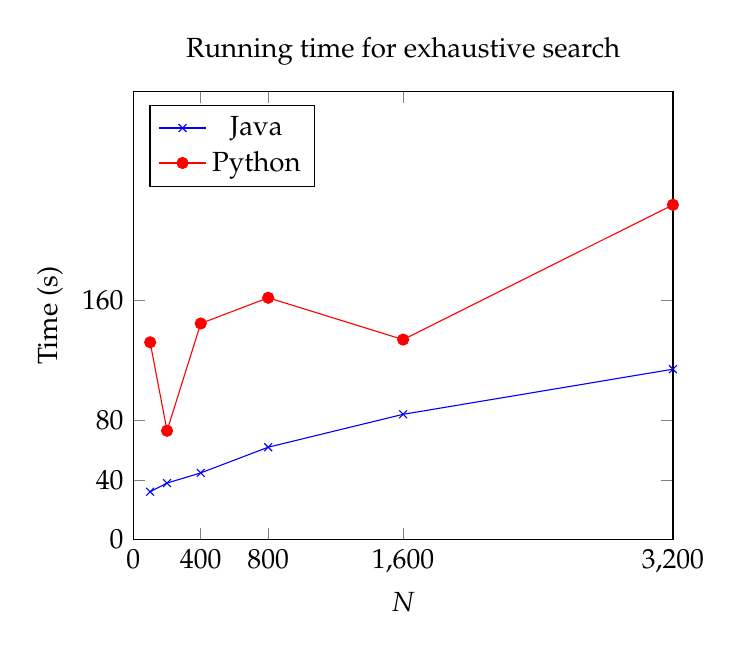
\begin{tikzpicture}
	\begin{axis}[
		title={Running time for exhaustive search},
		xlabel={$N$},
		ylabel={Time (s)},
		xmin=0, xmax=3200,
		ymin=0, ymax=300,
		xtick={0,400, 800, 1600,3200},
		ytick={0,40,80,160},
		legend pos=north west,
		%ymajorgrids=true,
		%grid style=dashed,
	]
	\addplot[ color=blue, mark=x, ]
	coordinates { (100,32)(200,37.8)(400,44.6)(800,61.8)(1600,83.8)(3200,114) };
	\addplot[ color=red, mark=*, ]
	coordinates { (100,132)(200,72.8)(400,144.6)(800,161.8)(1600,133.8)(3200,224) };
	\legend{Java, Python}
	\end{axis}
\end{tikzpicture}

\subsection{Improvements}

Using the binary search-based idea sketeched in [SW, 1.4] for the Three-sum problem, we can improve our running time to $\sim N^3\log N$. \sidenote{Correct as necessary. If instead you’ve figured out how to do it even faster, rewrite the whole sentence so as to explain what you do.}

The following table reports our maximum running times on the test inputs. [$\cdots$]

The following log--log plot shows these values graphically, note that the points are on a line of slope [$\cdots$].

\end{document}

